\documentclass{scrartcl}

\usepackage[linear]{handout}
\usepackage{bbm}
\usepackage{circuitikz}
% \usepackage{mlmodern}
% \usepackage{gfsartemisia}
\ihead{\sffamily\bfseries\footnotesize{Experiment 04}}
\ohead{\sffamily\footnotesize\textbf{}} 

\title{
        \Large\textsc{PH3204: Electronics Lab} \\
        \vspace{10pt}
        % \Large\textsc{Experiment 02} \\
        % \vspace{0.1cm}
        \Huge \textbf{Study of Boolean Algebra using Logic Gates} \\
}

% \subtitle{}

\author{Sabarno Saha \\ \texttt{22MS037} \\ Grp. B-10}

\date{\normalsize
        \textit{Indian Institute of Science Education and Research, Kolkata, \\
        Mohanpur, West Bengal, 741246, India.}
        % \vspace{10pt}
        % \today
}
\newcommand{\1}{\mathbbm{1}}
\newcommand{\ichi}{\tilde{\chi}}
\newcommand{\irho}{\tilde{\rho}}
\newcommand{\ihsr}{\tilde{H}_{SR}}
\newcommand{\G}{\Gamma}
\newcommand{\iG}{\tilde{\Gamma}}
\newcommand{\is}{\tilde{s}}
\newcommand{\h}{\mathbb{H}}
\newcommand{\nbar}{\bar{n}}

\renewcommand{\arraystretch}{1.5} % Increase row height
\graphicspath{{./code/}}

\begin{document}
\maketitle
\tableofcontents
\section{Aim}
In this experiment, we aim to study the basic laws of Boolean algebra using logic gates. The Logic gates we will be using are
AND, OR, NOT, NAND, NOR, and XOR gates. We will also study the properties of these gates and their applications in digital circuits. Then 
we will build a few circuits using these gates and verify their truth tables.
\section{Theory}
Boolean algebra is just the study of functions that map binary strings to either 0 or 1. The basic operations in Boolean algebra are \\
    AND: $Q = A \cdot B$ \hfill 
    OR: $Q = A + B$ \hfill 
    NOT: $Q = \overline{A}$ \\
We will be studying the properties of these gates and their applications in digital circuits. We will also study the NAND, NOR, and XOR gates.
\subsection{Gates}
\subsubsection{AND Gate}
The AND gate is a digital logic gate that implements logical multiplication. We represent the AND Gate using 
$Q = A \cdot B = AB$.
It behaves according to the trieeestd uth table shown below:
\begin{figure}[H]
        \centering
        \begin{subfigure}[b]{0.45\textwidth}
                \centering
                \begin{tabular}{|c|c|c|}
                        \hline
                        A & B & Q=AB \\
                        \hline
                        0 & 0 & 0 \\
                        0 & 1 & 0 \\
                        1 & 0 & 0 \\
                        1 & 1 & 1 \\
                        \hline
                \end{tabular}
                \caption{Truth Table of AND Gate}
        \end{subfigure}
        \hfill
        \begin{subfigure}{0.45\textwidth}
                \centering
                \begin{circuitikz}
                        \draw (0,0) node[ieeestd and port] (myand) {}
                        (myand.in 1) node[left] {A}
                        (myand.in 2) node[left] {B}
                        (myand.out) node[right] {Q};
                \end{circuitikz}
                \caption{Symbol of AND Gate}
        \end{subfigure}
        \caption{Truth Table and Symbol of AND Gate}
\end{figure}
We use the IC 7408 to implement the AND gate.
\subsubsection{OR Gate}
The OR Gate is a digital logic gate that implements logical addition. We represent the OR Gate using $Q = A + B$. The 
truth table for the OR gate is shown below:
\begin{figure}[H]
        \centering
        \begin{subfigure}{0.45\textwidth}
                \centering
                \begin{tabular}{|c|c|c|}
                        \hline
                        A & B & Q=A+B \\
                        \hline
                        0 & 0 & 0 \\
                        0 & 1 & 1 \\
                        1 & 0 & 1 \\
                        1 & 1 & 1 \\
                        \hline
                \end{tabular}
                \caption{Truth Table of OR Gate}
        \end{subfigure}
        \hfill
        \begin{subfigure}{0.45\textwidth}
                \centering
                \begin{circuitikz}
                        \draw (0,0) node[ieeestd or port] (myor) {}
                        (myor.in 1) node[left] {A}
                        (myor.in 2) node[left] {B}
                        (myor.out) node[right] {Q};
                \end{circuitikz}
                \caption{Symbol of OR Gate}
        \end{subfigure}
        \caption{Truth Table and Symbol of OR Gate}
\end{figure}
We use the IC 7432 to implement the OR gate.
\subsubsection{NOT Gate}
The NOT Gate is a digital logic gate that implements logical negation. We represent the NOT Gate using $Q = \overline{A}$. The
truth table for the NOT gate is shown below:
\begin{figure}[H]
        \centering
        \begin{subfigure}{0.45\textwidth}
                \centering
                \begin{tabular}{|c|c|}
                        \hline
                        A & Q=$\overline{A}$ \\
                        \hline
                        0 & 1 \\
                        1 & 0 \\
                        \hline
                \end{tabular}
                \caption{Truth Table of NOT Gate}
        \end{subfigure}
        \hfill
        \begin{subfigure}{0.45\textwidth}
                \centering
                \begin{circuitikz}
                        \draw (0,0) node[ieeestd not port] (mynot) {}
                        (mynot.in) node[left] {A}
                        (mynot.out) node[right] {Q};
                \end{circuitikz}
                \caption{Symbol of NOT Gate}
        \end{subfigure}
        \caption{Truth Table and Symbol of NOT Gate}
\end{figure}
We use the IC 7404 to implement the NOT gate.
\subsubsection{NAND Gate}
The NAND Gate is a digital logic gate that implements the logical negation of the logical multiplication. We represent the NAND Gate using $Q = \overline{AB}$. 
This gate just inverts the output of the AND gate. The truth table for the NAND gate is shown below:
\begin{figure}[H]
        \centering
        \begin{subfigure}{0.45\textwidth}
                \centering
                \begin{tabular}{|c|c|c|}
                        \hline
                        A & B & Q=$\overline{AB}$ \\
                        \hline
                        0 & 0 & 1 \\
                        0 & 1 & 1 \\
                        1 & 0 & 1 \\
                        1 & 1 & 0 \\
                        \hline
                \end{tabular}
                \caption{Truth Table of NAND Gate}
        \end{subfigure}
        \hfill
        \begin{subfigure}{0.45\textwidth}
                \centering
                \begin{circuitikz}
                        \draw (0,0) node[ieeestd nand port] (mynand) {}
                        (mynand.in 1) node[left] {A}
                        (mynand.in 2) node[left] {B}
                        (mynand.out) node[right] {Q};
                \end{circuitikz}
                \caption{Symbol of NAND Gate}
        \end{subfigure}
        \caption{Truth Table and Symbol of NAND Gate}
\end{figure}
We use the IC 7400 to implement the NAND gate.

\subsubsection{NOR Gate}
The NOR Gate is a digital logic gate that implements the logical negation of the logical addition. We represent the NOR Gate using $Q = \overline{A+B}$.
This gate just inverts the output of the OR gate. The truth table for the NOR gate is shown below:
\begin{figure}[H]
        \centering
        \begin{subfigure}{0.45\textwidth}
                \centering
                \begin{tabular}{|c|c|c|}
                        \hline
                        A & B & Q=$\overline{A+B}$ \\
                        \hline
                        0 & 0 & 1 \\
                        0 & 1 & 0 \\
                        1 & 0 & 0 \\
                        1 & 1 & 0 \\
                        \hline
                \end{tabular}
                \caption{Truth Table of NOR Gate}
        \end{subfigure}
        \hfill
        \begin{subfigure}{0.45\textwidth}
                \centering
                \begin{circuitikz}
                        \draw (0,0) node[ieeestd nor port] (mynor) {}
                        (mynor.in 1) node[left] {A}
                        (mynor.in 2) node[left] {B}
                        (mynor.out) node[right] {Q};
                \end{circuitikz}
                \caption{Symbol of NOR Gate}
        \end{subfigure}
        \caption{Truth Table and Symbol of NOR Gate}
\end{figure}
We use the IC 7402 to implement the NOR gate.
\subsubsection{XOR Gate}
The XOR Gate is a digital logic gate that implements the logical addition modulo 2. We represent the XOR Gate using $Q = A \oplus B$. The 
boolean expression for the XOR gate is $Q = A\overline{B} + \overline{A}B$.
The truth table for the XOR gate is shown below:
\begin{figure}[H]
        \centering
        \begin{subfigure}{0.45\textwidth}
                \centering
                \begin{tabular}{|c|c|c|}
                        \hline
                        A & B & Q=$A \oplus B$ \\
                        \hline
                        0 & 0 & 0 \\
                        0 & 1 & 1 \\
                        1 & 0 & 1 \\
                        1 & 1 & 0 \\
                        \hline
                \end{tabular}
                \caption{Truth Table of XOR Gate}
        \end{subfigure}
        \hfill
        \begin{subfigure}{0.45\textwidth}
                \centering
                \begin{circuitikz}
                        \draw (0,0) node[ieeestd xor port] (myxor) {}
                        (myxor.in 1) node[left] {A}
                        (myxor.in 2) node[left] {B}
                        (myxor.out) node[right] {Q};
                \end{circuitikz}
                \caption{Symbol of XOR Gate}
        \end{subfigure}
        \caption{Truth Table and Symbol of XOR Gate}
\end{figure}
We use the IC 7486 to implement the XOR gate.
\subsection{Pin diagrams of ICs}
The ICs used here are the 74LSXX series, where LS stands for Low Power Schottky. The pin diagrams of the ICs are shown below:
\begin{figure}[H]
        \centering
        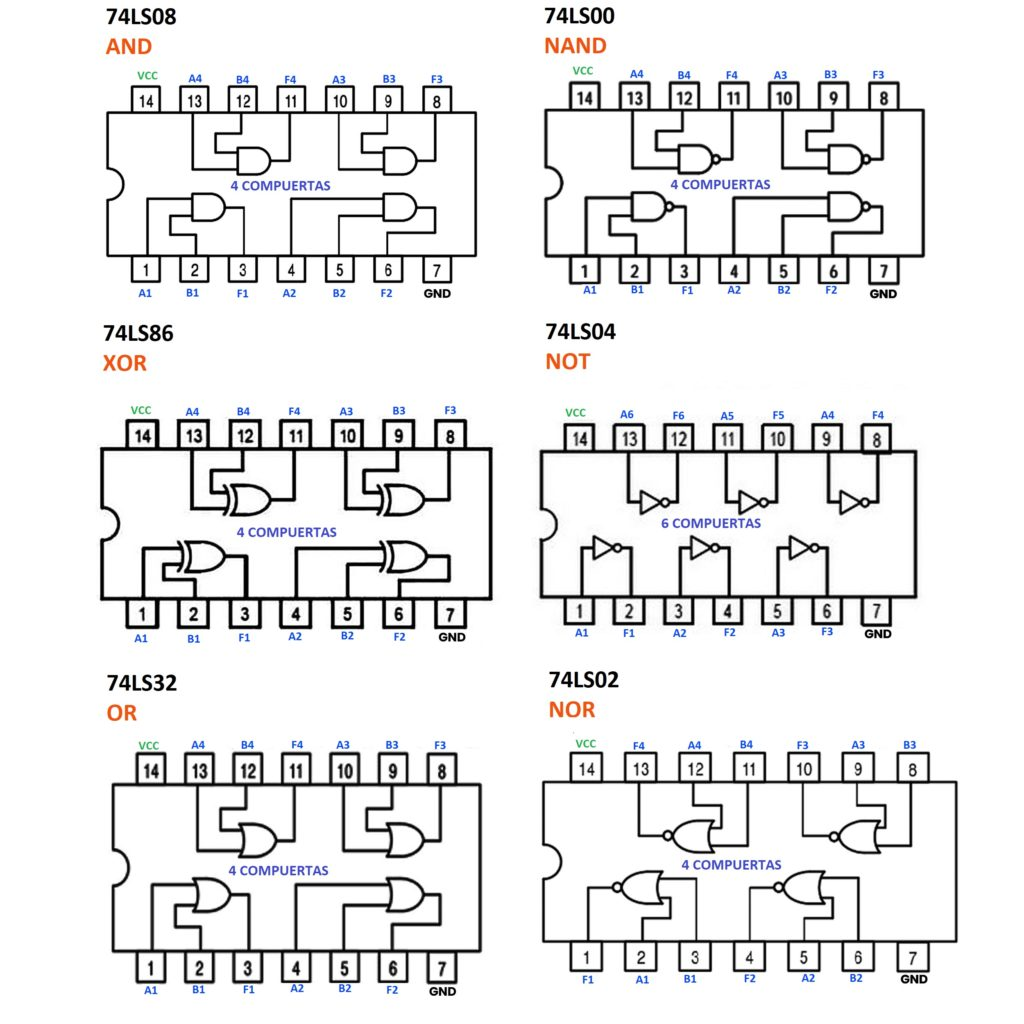
\includegraphics[width=0.8\textwidth]{gates.png}
        \caption{Pin Diagram of IC 7400. (Source : The Internet)}
\end{figure}
\section{Experiment}
\subsection{Example 1}
\begin{figure}[H]
        \centering
        \begin{circuitikz}
    % Draw the AND gate
    \node[ieeestd and port] (and) at (0,0) {AND};

    % Draw the OR gate
    \node[ieeestd or port] (or) at (0,-4) {OR};

    % Draw the NAND gate
    \node[ieeestd nand port] (nand) at (3,-2) {NAND};

    % Draw the NOR gate
    \node[ieeestd nor port] (nor) at (6,-1) {NOR};

    % Draw the XOR gate
    \node[ieeestd xor port] (xor) at (6,-3.7) {XOR};

    % Draw the final AND gate
    \node[ieeestd and port] (final_and) at (9,-2) {AND};

    % Connect the AND gate to the NAND gate
    \draw (and.in 2) -- ++(-0,-1) |- (nand.in 1);
    \draw (and.out) -- ++(0.5,0) |- (nor.in 1);

    % Connect the OR gate to the NAND gate
    \draw (or.out) -- ++(0.5,0) |- (nand.in 2);
    \draw (or.out) -- ++(0.5,0) |- (xor.in 2);

    % Connect the NAND gate to the NOR gate
    \draw (nand.out) -- ++(0.5,0) |- (nor.in 2);

    % Connect the NAND gate to the XOR gate
    \draw (nand.out) -- ++(0.5,0) |- (xor.in 1);

    % Connect the NOR gate to the final AND gate
    \draw (nor.out) -- ++(0.5,0) |- (final_and.in 1);

    % Connect the XOR gate to the final AND gate
    \draw (xor.out) -- ++(0.5,0) |- (final_and.in 2);

    % Label inputs and outputs
    \draw (and.in 1) -- ++(-1,0) node[left] {A};
    \draw (and.in 2) -- ++(-1,0) node[left] {B};
    \draw (or.in 1) -- ++(-1,0) node[left] {C};
    \draw (or.in 2) -- ++(-1,0) node[left] {D};
    \draw (final_and.out) -- ++(1,0) node[right] {Q};
\end{circuitikz}
        \caption{Circuit Diagram of the given circuit}
\end{figure}
The Simplified boolean expression for the circuit is $Q = \overline{A}B(C+D)$. The truth table for the circuit is shown below:
\begin{table}[H]
    \centering
    \caption{Truth Table for \( \mathrm{Q} = \overline{\mathrm{A}}\mathrm{B}(\mathrm{C + D}) \)}
    \vspace{0.2cm}
    \begin{tabular}{|c|c|c|c||c|||c|c|c|c||c|}
    \hline
    \textbf{A} & \textbf{B} & \textbf{C} & \textbf{D} & \textbf{Q} & \textbf{A} & \textbf{B} & \textbf{C} & \textbf{D} & \textbf{Q}\\
    \hline
    0 & 0 & 0 & 0 & 0 & 1 & 0 & 0 & 0 & 0 \\
    0 & 0 & 0 & 1 & 0 & 1 & 0 & 0 & 1 & 0 \\
    0 & 0 & 1 & 0 & 0 & 1 & 0 & 1 & 0 & 0 \\
    0 & 0 & 1 & 1 & 0 & 1 & 0 & 1 & 1 & 0 \\
    0 & 1 & 0 & 0 & 0 & 1 & 1 & 0 & 0 & 0 \\
    0 & 1 & 0 & 1 & 1 & 1 & 1 & 0 & 1 & 0 \\
    0 & 1 & 1 & 0 & 1 & 1 & 1 & 1 & 0 & 0 \\
    0 & 1 & 1 & 1 & 1 & 1 & 1 & 1 & 1 & 0 \\
    \hline
    \end{tabular}
\end{table}

\subsection{Example 2}
\begin{figure}[H]
        \centering
        \begin{circuitikz}
    % Draw the AND gate
    \node[ieeestd and port] (and) at (0,0) {AND};

    % Draw the OR gate
    \node[ieeestd nand port] (nand) at (0,-4) {NAND};

    % Draw the XOR gate
    \node[ieeestd xor port] (xor) at (3,-2) {XOR};

    % Draw the NOR gate
    \node[ieeestd nor port] (nor) at (6,-1) {NOR};

    % Draw the final AND gate
    \node[ieeestd and port] (final_and) at (6,-3.72) {AND};

    % Draw the OR gate
    \node[ieeestd or port] (or) at (9,-2) {OR};

    % Connect the AND gate to the NAND gate
    \draw (and.in 2) -- ++(-0,-1) |- (xor.in 1);
    \draw (and.out) -- ++(0.5,0) |- (nor.in 1);

    % Connect the OR gate to the NAND gate
    \draw (nand.out) -- ++(0.5,0) |- (xor.in 2);
    \draw (nand.out) -- ++(0.5,0) |- (final_and.in 2);

    % Connect the NAND gate to the NOR gate
    \draw (xor.out) -- ++(0.5,0) |- (nor.in 2);

    % Connect the NAND gate to the XOR gate
    \draw (xor.out) -- ++(0.5,0) |- (final_and.in 1);

    % Connect the NOR gate to the final AND gate
    \draw (final_and.out) -- ++(0.5,0) |- (or.in 2);

    % Connect the XOR gate to the final AND gate
    \draw (nor.out) -- ++(0.5,0) |- (or.in 1);

    % Label inputs and outputs
    \draw (and.in 1) -- ++(-1,0) node[left] {A};
    \draw (and.in 2) -- ++(-1,0) node[left] {B};
    \draw (nand.in 1) -- ++(-1,0) node[left] {C};
    \draw (nand.in 2) -- ++(-1,0) node[left] {D};
    \draw (or.out) -- ++(1,0) node[right] {Q};
\end{circuitikz}
        \caption{Circuit Diagram of the given circuit}
\end{figure}
The Simplified boolean expression for the above circuit was found out to be
$\mathrm{Q = \overline{B} + \overline{A}B(\overline{C} + \overline{D})}$
\begin{table}[H]
    \centering
    \caption{Truth Table for $Q = \overline{B} + \overline{A}B(\overline{C} + \overline{D})$ }
    \begin{tabular}{|c|c|c|c||c|||c|c|c|c||c|}
    \hline
        \textbf{A} & \textbf{B} & \textbf{C} & \textbf{D} & \textbf{Q} & \textbf{A} & \textbf{B} & \textbf{C} & \textbf{D} & \textbf{Q}\\ \hline
        0 & 0 & 0 & 0 & 1 & 1 & 0 & 0 & 0 & 1 \\
        0 & 0 & 0 & 1 & 1 & 1 & 0 & 0 & 1 & 1 \\
        0 & 0 & 1 & 0 & 1 & 1 & 0 & 1 & 0 & 1 \\
        0 & 0 & 1 & 1 & 1 & 1 & 0 & 1 & 1 & 1 \\
        0 & 1 & 0 & 0 & 1 & 1 & 1 & 0 & 0 & 0 \\
        0 & 1 & 0 & 1 & 1 & 1 & 1 & 0 & 1 & 0 \\
        0 & 1 & 1 & 0 & 1 & 1 & 1 & 1 & 0 & 0 \\
        0 & 1 & 1 & 1 & 0 & 1 & 1 & 1 & 1 & 0 \\
        \hline
    \end{tabular}
\end{table}
\subsection{Example 3}
\begin{figure}[H]
        \centering
        \begin{circuitikz}
    % Draw the AND gate
    \node[ieeestd nor port] (nor) at (0,0) {NOR};

    % Draw the OR gate
    \node[ieeestd and port] (and) at (0,-4) {AND};

    % Draw the NAND gate
    \node[ieeestd or port] (or) at (3,-2) {OR};

    % Draw the NOR gate
    \node[ieeestd nand port] (nand) at (6,-1) {NAND};

    % Draw the XOR gate
    \node[ieeestd and port] (and2) at (6,-3.72) {AND};

    % Draw the final AND gate
    \node[ieeestd xor port] (xor) at (9,-2) {XOR};

    % Connect the AND gate to the NAND gate
    \draw (nor.in 2) -- ++(-0,-1) |- (or.in 1);
    \draw (nor.out) -- ++(0.5,0) |- (nand.in 1);

    % Connect the OR gate to the NAND gate
    \draw (and.out) -- ++(0.5,0) |- (or.in 2);
    \draw (and.out) -- ++(0.5,0) |- (and2.in 2);

    % Connect the NAND gate to the NOR gate
    \draw (or.out) -- ++(0.5,0) |- (nand.in 2);

    % Connect the NAND gate to the XOR gate
    \draw (or.out) -- ++(0.5,0) |- (and2.in 1);

    % Connect the NOR gate to the final AND gate
    \draw (nand.out) -- ++(0.5,0) |- (xor.in 1);

    % Connect the XOR gate to the final AND gate
    \draw (and2.out) -- ++(0.5,0) |- (xor.in 2);

    % Label inputs and outputs
    \draw (nor.in 1) -- ++(-1,0) node[left] {A};
    \draw (nor.in 2) -- ++(-1,0) node[left] {B};
    \draw (and.in 1) -- ++(-1,0) node[left] {C};
    \draw (and.in 2) -- ++(-1,0) node[left] {D};
    \draw (xor.out) -- ++(1,0) node[right] {Q};
\end{circuitikz}
        \caption{Circuit Diagram of the given circuit}
\end{figure}
The simplified boolean expression for the above circuit was found out to be
$\mathrm{Q = \overline{A}\ \overline{B}+ \overline{C} + \overline{D}}$.
\begin{table}[H]
        \centering
        \caption{Truth Table for \(\mathrm{ \mathrm{Q} = \overline{A}\,\overline{B} + \overline{D} + \overline{C} }\)}
        \vspace{0.2cm}
        \begin{tabular}{|c|c|c|c||c|||c|c|c|c||c|}
        \hline
        \textbf{A} & \textbf{B} & \textbf{C} & \textbf{D} & \textbf{Q} & \textbf{A} & \textbf{B} & \textbf{C} & \textbf{D} & \textbf{Q} \\
        \hline
        0 & 0 & 0 & 0 & 1 & 1 & 0 & 0 & 0 & 1 \\
        0 & 0 & 0 & 1 & 1 & 1 & 0 & 0 & 1 & 1 \\
        0 & 0 & 1 & 0 & 1 & 1 & 0 & 1 & 0 & 1 \\
        0 & 0 & 1 & 1 & 1 & 1 & 0 & 1 & 1 & 0 \\
        0 & 1 & 0 & 0 & 1 & 1 & 1 & 0 & 0 & 1 \\
        0 & 1 & 0 & 1 & 1 & 1 & 1 & 0 & 1 & 1 \\
        0 & 1 & 1 & 0 & 1 & 1 & 1 & 1 & 0 & 1 \\
        0 & 1 & 1 & 1 & 0 & 1 & 1 & 1 & 1 & 0 \\
        \hline
        \end{tabular}
\end{table}
\section{Results}
The truth tables for the individual gates were verified and the simplified boolean expressions for the circuits were found out.
Then the truth tables were also experimentally verified.
\section{Conclusion}
We conclude by verifying the truth tables of the individual gates and the circuits.
\end{document}
